\subsection{Astrobiology}
\label{sec:AstrobiologyBackground}

Extremophiles are microorganisms that thrive in physically and/or chemically extreme conditions, which are detrimental to most of life on Earth as we know it. These organisms and microbes have been found everywhere, from deep underwater volcano vents to buried ice lakes in Antarctica \cite{Extremophiles}. 

Fungi and bacterial spores have also been found in the stratosphere. Today, the most common altitudes for organism and microbe collection in the atmosphere are in the range of approximately 10 km to 20 km above Earth’s surface. As illustrated in the table below, very little data exists on microbiological samples captured in the stratosphere \cite{Extremophiles}. Conditions at altitudes of 30km to 40km are extreme in temperature, pressure and radiation exposure. Arguably, each successful collection expedition, of at least 30 km into the upper atmosphere, provides information that can be useful in determining what life forms can exist inside and outside of Earth’s biosphere. Additionally, RNA analysis of the organisms and microbes can provide useful insight pertaining to their ability to survive in an environment with elevated levels of radiation.  

 Our experiment focuses on designing a more energy efficient compact collection apparatus that refining our sanitization procedures for preflight assembly, post flight disassembly, and RNA sequencing preparation. We also want to test the effectiveness of rotating filters to stationary ones. The samples we will collect play an important role in expanding our knowledge about Earth’s biosphere. Future studies could produce meaningful contributions to the fields of gene therapy, RNA interface, and cosmic shielding; and provide valuable insight about how life can be distributed on Earth, and ultimately, through outer-space.

%\begin{figure}[H]
%\centering
%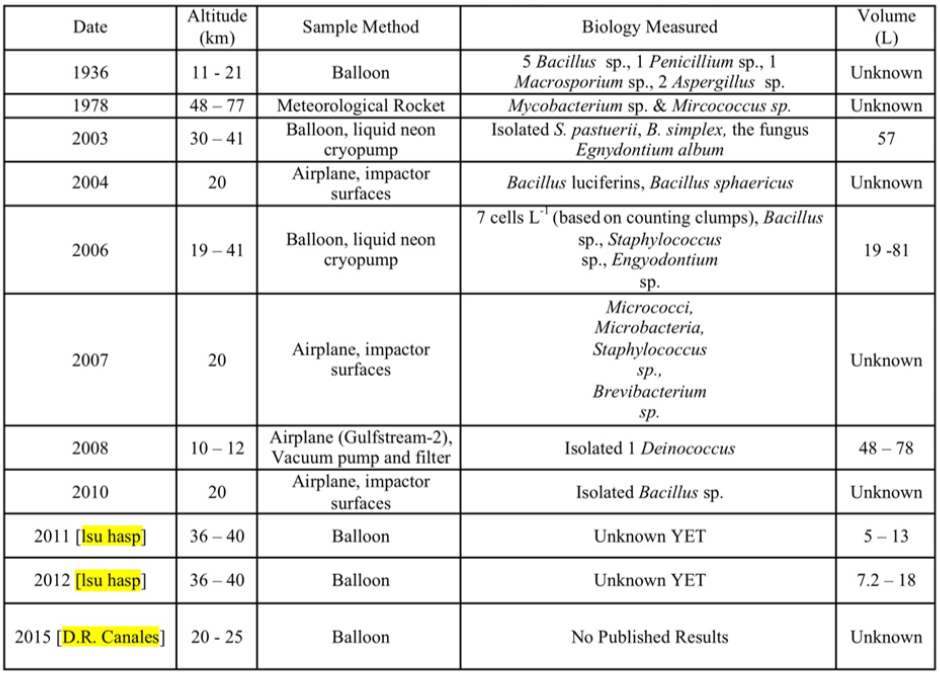
\includegraphics[width=1\textwidth]{./Figures/AstroChart.PNG}
%\caption{}
%\label{fig:AstroHist}
%\end{figure} 

Our experiment is an attempt to further develop our technique for capturing microorganisms in the upper atmosphere, as demonstrated during our 2017~\cite{SORA1} flight; which was inspired by the LSU HASP 2011, 2012, 2013 flights~\cite{LSU} and from research by D.R. Canales~\cite{Canales}.  This flight will help confirm the results from our first and second flights\cite{SORA2}.  We will use a rotating arm mechanism to sample the air for microorganisms through the use of fluropore membrane filters. The samples we hope to collect are an important part to expanding our understanding of Earth's biosphere. Further studies could provide more insight on how life can be distributed on Earth, and ultimately, through outer-space.

\begin{table}[!ht]
  \centering
  \caption{History of Microbiological Sampling of the stratosphere~\cite{SORA1}.} 
  \bigskip
  \begin{tabular}{c c c p{6cm} c}
    \hline
    \hline
    \multicolumn{1}{c}{\bfseries Date} & \minitab{c}{\bf Altitude}{\bf (km)} &  \multicolumn{1}{c}{\bfseries Sample Method} & \multicolumn{1}{p{6cm}}{\bfseries Biology Measured} & \multicolumn{1}{c}{\bfseries Volume} \\
    \hline
    1936 & 11 - 12 & Balloon			 		& \minitab{l}{5 Bacillus sp., 1 Penicillium sp.,}{1 Macrosporium sp., 2 Aspergillus sp.} 	  & $Unknown$ \\ \hline
    1978 & 48 - 77 & Meteorological rocket 		        & \minitab{l}{}\par Mycobacterium sp., Mircococcus sp.					          & $Unknown$ \\ \hline
    2003 & 30 - 41 & Balloon, liquid neon cryopump	        & \minitab{l}{Isolated S. pastuerii, B. simplex,}{the fungus, Egnydontium album}       		  & $57$      \\ \hline
    2004 & 20	   & Airplane, impactor surfaces 	        & \minitab{l}{}\par Bacillus luciferins, Bacillus sphaericus			                  & $Unknown$ \\ \hline
    2006 & 19 - 41 & Balloon, liquid neon cryopump              & \minitab{l}{7 cells L-1 (counting clumps), Bacillus sp.,}{Staphylococcus sp., Engyodontium sp.} & $19-81$   \\ \hline
    2007 & 20	   & Airplane, impactor surfaces 	        & \minitab{l}{Micrococci, Microbacteria,}{Staphylococcus sp., Brevibacterium sp.}    		  & $Unknown$ \\ \hline
    2010 & 20	   & Airplane, impactor surfaces                & \minitab{l}{}\par Isolated Bacillus sp.							  & $Unknown$ \\ \hline
    2017 & 32	   & Balloon, liquid medium w/ vacuum pump	& \minitab{l}{}\par Multiple findings~\cite{SORA1}					          & $Unknown$ \\ \hline
    2018 & 32	   & Balloon, liquid medium w/ vacuum pump	& \minitab{l}{}\par Inconclusive~\cite{SORA2}							  & $Unknown$ \\ \hline
  \end{tabular}
  \label{tab:AstrobiologyTable}
  \medskip
\end{table}
